\documentclass[a4paper,oneside,12pt]{article}

% --- Packages ---
\usepackage[ngerman]{babel} % Deutsche Spracheinstellungen
\usepackage{amsmath}        % Mathematische Formeln
\usepackage{amsfonts}       % Mathematische Schriftarten
\usepackage{amssymb}        % Zusätzliche mathematische Symbole
\usepackage{graphicx}       % Bilder einfügen
%\usepackage[colorlinks=true, allcolors=blue]{hyperref} % Verlinkungen mit Farben
\usepackage[hidelinks]{hyperref} % Verlinkungen ohne Umrandung
\usepackage[tmargin=1in,bmargin=1in,lmargin=1.25in,rmargin=1.25in]{geometry} % Seitenränder einstellen
\usepackage{setspace}       % Zeilenabstand anpassen
\onehalfspacing             % 1,5-zeiliger Abstand
\bibliographystyle{unsrtdin}   % Stil für Literaturverzeichnis
\usepackage{siunitx}        % SI-Einheiten und Zahlenformatierung
\usepackage{xcolor}         % Farben verwenden
\usepackage{caption}        % Bildunterschriften anpassen
\usepackage{subcaption}     % Mehrere Bilder nebeneinander
\usepackage{multirow}       % Verbundene Tabellenzeilen
\usepackage{booktabs}       % Stilvolle Tabellen
\usepackage{fancyhdr}       % Kopf- und Fußzeilen anpassen
\usepackage{lipsum}         % Platzhaltertext
\usepackage{circuitikz}     % Schaltungsdiagramme
\usepackage{pgfplots}       % Diagramme erstellen
\pgfplotsset{compat=1.18}   % Aktuelle Kompatibilitätsversion
\usepackage{pgfplotstable}  % CSV-Daten importieren
\usepackage{array}          % Erweiterte Tabellenspalten
\usepackage{float}          % Steuerung von Gleitobjekten
\usepackage{cleveref}       % Intelligente Referenzen
\usepackage{icomma}         % Korrekte Dezimaltrennung

% --- Dokument beginnt hier ---
\begin{document}

% Definitionen laden
% --- Deckblatt Definitionen ---
\def\labtitle{Elektronische Produktentwicklung} % Titel des Labors
\def\labcode{MECH-B-4-AED-EPE1-ILV} % Code des Labors
\def\labname{} % Name des Labors
\def\labnum{Nummer der Laborübung} % Nummer der Laborübung
\def\labdate{Datum Labor} % Datum des Labors
\def\study{Bachelor: Mechatronik Design and Innovation} % Studienrichtung
\def\studygroup{} % Studiengruppe
\def\term{4.} % Semesterzahl
\def\lecturer{Rene Feldkircher} % Dozent
\def\group{BA-MECH-24} % Studiengruppe
\def\student{Seyam Mir Afghan, Elham Mir Afghan, Nils Brieger, Benedikt Motzet} % Studierende
\def\contributor{}
\def\litname{literatur} % Literaturverzeichnis

% --- Kopf- und Fußzeile definieren ---
\fancyhf{} % Alle Kopf- und Fußzeilenfelder leeren
\fancyhead[L]{\labtitle} % Kopfzeile links
\fancyhead[C]{} % Kopfzeile zentriert
\fancyhead[R]{\labname} % Kopfzeile rechts
\renewcommand{\headrulewidth}{0.4pt} % Trennlinie oben
\fancyfoot[L]{\thepage} % Seitenzahl links
\fancyfoot[R]{{\footnotesize\student}} % Studierende rechts
\renewcommand{\footrulewidth}{0.4pt} % Trennlinie unten
\setlength{\headheight}{14.49998pt} % Kopfzeilenhöhe anpassen
\addtolength{\topmargin}{-2.49998pt} % Seitenrand ausgleichen

% --- Tabellenhöhen anpassen ---
\renewcommand{\arraystretch}{1.2} % Zeilenhöhe für Tabellen erhöhen

% --- Bildunterschriften anpassen ---
\captionsetup{belowskip=12pt, aboveskip=4pt} % Abstand über und unter Bildunterschriften
\captionsetup{font=footnotesize} % Schriftgröße für Bildunterschriften

% --- Absatzformatierung ---
\setlength{\parindent}{0em} % Kein Einzug bei Absätzen
\setlength{\parskip}{1.5ex plus0.5ex minus0.5ex} % Abstand zwischen Absätzen

% --- Überfüllungswarnungen minimieren ---
\tolerance = 9999
\sloppy

% --- SI-Einheiten (siunitx Einstellungen) ---
\sisetup{
    output-decimal-marker={,}, % Komma als Dezimaltrennzeichen
    per-mode=reciprocal, % Brüche im Kehrwertmodus
    exponent-product=\cdot, % Malzeichen für Exponenten
    retain-explicit-plus, % Pluszeichen beibehalten
    range-phrase = {\dots}, % Bereich mit "..."
    separate-uncertainty, % Unsicherheit getrennt anzeigen
    list-separator={; }, % Listentrenner
    list-final-separator={; } % Abschließender Listentrenner
}

% --- Diagrammeinstellungen (pgfplots) ---
\pgfplotsset{
    /pgf/number format/use comma, % Komma als Dezimaltrennzeichen
    /pgf/number format/.cd, set thousands separator={\,} % Tausendertrennzeichen
}
 

% Deckblatt einfügen
\pagestyle{plain} % Einfache Kopf- und Fußzeile
\input{Sections/deckblatt.tex}

% Wechsel zu Serifenschrift
%\rmfamily

\pagestyle{fancy} % Kopf- und Fußzeilen aktivieren

\begin{spacing}{0.6}
% --- Inhaltsverzeichnis ---
\pagenumbering{Roman} % Römische Nummerierung
\setcounter{page}{2} % Beginnt bei Seite II
\tableofcontents % Inhaltsverzeichnis
\newpage
\end{spacing}

%\pagestyle{fancy} % Kopf- und Fußzeilen aktivieren

% --- Arabische Nummerierung für Hauptkapitel ---
\pagenumbering{arabic} % Arabische Nummerierung
\setcounter{page}{1} % Beginnt bei Seite 1

% Kapitel einfügen

\section{Einleitung}
Im Elektrotechnik-Labor werden grundlegende Prinzipien von Gleich- und Wechselstromkreisen untersucht. Ziel ist es, die Eigenschaften dieser Schaltungen zu analysieren, ihr Verhalten unter verschiedenen Bedingungen zu beobachten und präzise Messungen mit spezifischen Geräten durchzuführen. Der Schwerpunkt liegt dabei auf der praktischen Anwendung der theoretischen Grundlagen.

Einige der theoretischen Grundlagen sowie ergänzende Informationen zur Analyse werden aus Fachliteratur entnommen, insbesondere aus den Werken von Marinescu et al. (\textit{Elektrotechnik für Studium und Praxis} \cite{marinescu2021}, \textit{Elektrische und magnetische Felder} \cite{marinescu2012}) sowie Böhmer et al. (\textit{Elemente der angewandten Elektronik} \cite{böhmer2114}).

Im Folgenden sind die für den Versuch verwendeten Geräte aufgelistet:

\begin{itemize}
    \item \textbf{PC-Electronic-Board (hps Systemtechnik GmbH)}: Lern- und Experimentiersystem für die Elektrotechnik.
    \item \textbf{Digitalmultimeter Amprobe AM-510-EUR}: Zur präzisen Messung von elektrischen Größen wie Spannung, Strom und Widerstand.
    \item \textbf{Frequenzgenerator AIM-TTi TG1000}: Zur Erzeugung von Signalen unterschiedlicher Frequenz und Amplitude.
    \item \textbf{Keysight DSOX1102A}: Zweikanal-Oszilloskop zur Darstellung und Analyse von Signalverläufen.
    \item \textbf{Bananenstecker}: Zur sicheren und flexiblen Verbindung der Schaltungskomponenten.
\end{itemize}

Die für die Versuche verwendeten Schaltbilder und Aufbauanleitungen wurden der \textit{Praktikumsanleitung Labor Elektrotechnik} \cite{praktikumsanleitung2024} entnommen und direkt übernommen, um eine einheitliche Dokumentation zu gewährleisten.

Der \textbf{vollständige rechnerische Weg} zur Überprüfung der Ergebnisse ist im Anhang~\ref{appA} detailliert beschrieben.

\newpage

\section{Ohmsches Gesetz}

Das Ohmsche Gesetz gehört zu den grundlegenden Prinzipien der Elektrotechnik. Es beschreibt den linearen Zusammenhang zwischen der Spannung $U$, der Stromstärke $I$ und dem Widerstand $R$ in einem elektrischen Stromkreis. Dieser Zusammenhang wird durch die Gleichung \eqref{eq:Ohm'sche Gleichung} beschrieben:
\begin{equation} \label{eq:Ohm'sche Gleichung}
    U = I \cdot R
\end{equation}
Zur Veranschaulichung des Ohmschen Gesetzes wird die in Abbildung \ref{fig:K2A1} dargestellte Schaltung aufgebaut. In diesem Experiment wird zunächst die Stromstärke $I$ in Abhängigkeit von der Spannung $U$ bei einem konstanten Widerstand $R$ gemessen und die Ergebnisse in Tabelle \ref{tab:K2T1} dokumentiert. Anschließend wird die Stromstärke $I$ in Abhängigkeit vom Widerstand $R$ bei einer konstanten Spannung $U$ erfasst und in Tabelle \ref{tab:K2T2} aufgeführt.

Die Messdaten werden jeweils grafisch aufbereitet, um den Zusammenhang in Form von Kennlinien darzustellen (siehe Abbildung \ref{fig:K2A2} und Abbildung \ref{fig:K2A3}). Diese grafische Auswertung dient der Überprüfung der Gültigkeit des Ohmschen Gesetzes.
\begin{figure}[H]
    \centering
    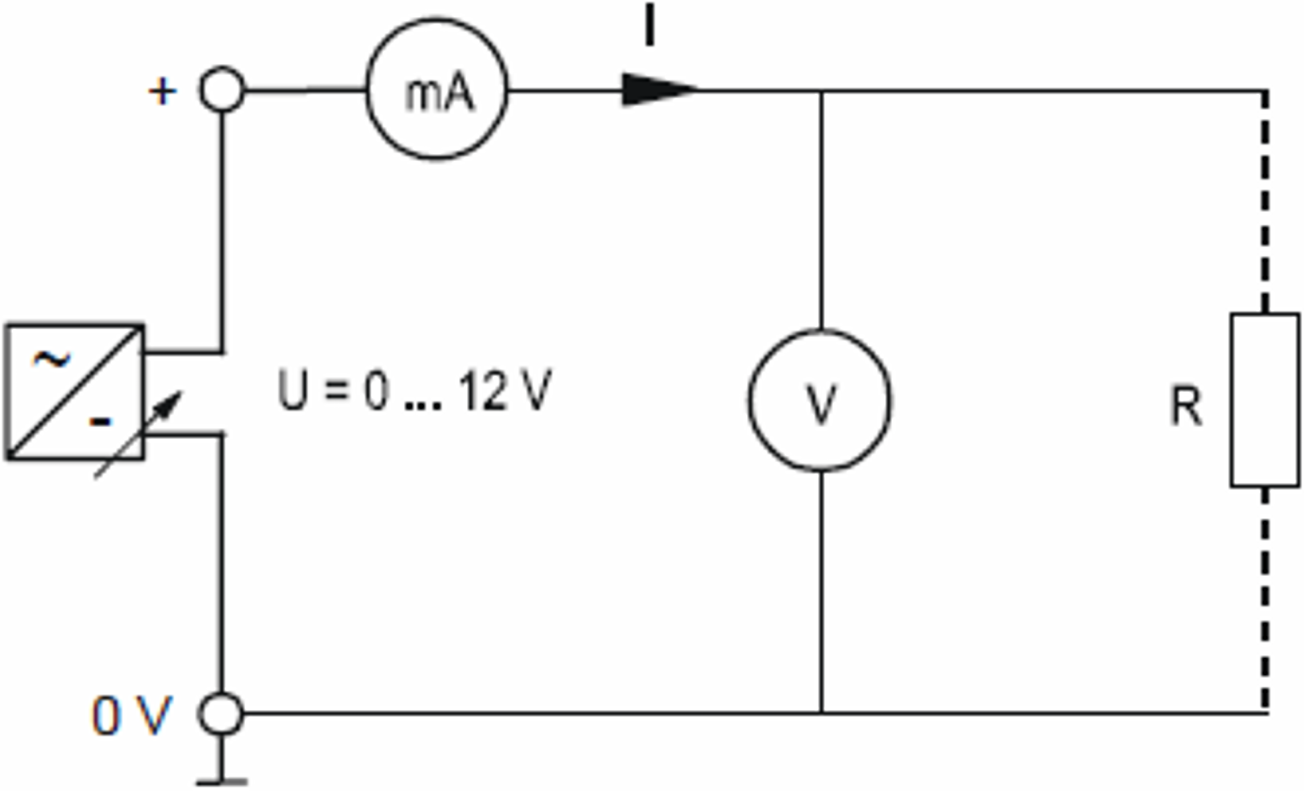
\includegraphics[width=0.5\textwidth]{Pictures/Kapitel2/Ohmsches Gesetz.png}
    \caption{Schematischer Aufbau des Stromkreises zur Untersuchung des Widerstands}
    \label{fig:K2A1}
\end{figure}

\subsection{Messwerte}
\begin{table}[H]
\centering
\caption{Gemessene Werte für $I$ in Abhängigkeit von $U$ bei konstantem $R$}
\begin{tabular}{ c c c c c c c c } % Abstand der Spalten
\toprule
    $U/\,\unit{V}$& 0 & 2 & 4 & 6 & 8 & 10 & 12\\
     \midrule
    $I/\,\unit{mA}$ bei $100\,\unit{\Omega}$&0,0 & 19,8 & 39,6 & 59,2 & 78,8 & 98,4 & 117,6\\
    $I/\,\unit{mA}$ bei $300\,\unit{\Omega}$& 0,0 & 6,1 & 12,2 & 18,3 & 24,5 & 30,7 & 36,8\\
    \bottomrule
\end{tabular}{}
\label{tab:K2T1}%Kapitel1 Ohmsches Gesetz Tabelle1
\end{table}{}

\begin{table}[H]
\centering
\caption{Gemessene Werte für $I$ in Abhängigkeit von $R$ bei konstanter $U$}
\begin{tabular}{ c c c c c c c } % Abstand der Spalten
\toprule
    $R/\,\unit{\Omega}$& 100 & 220 & 330 & 470 & 680 & 1000\\
     \midrule
    $I/\,\unit{mA}$ bei $\SI{12}{\V}$&118,20 & 54,30 & 36,87 & 25,64 & 17,76 & 12,24\\
    $I/\,\unit{mA}$ bei $\SI{8}{\V}$& 79,00 & 36,33 & 24,55 & 17,05 & 11,81 & 8,13\\
    $I/\,\unit{mA}$ bei $\SI{4}{\V}$& 39,60 & 18,19 & 12,29 & 8,53 & 5,90 & 4,06\\
    \bottomrule
\end{tabular}{}
\label{tab:K2T2}%Kapitel1 Ohmsches Gesetz Tabelle2
\end{table}{}

\vspace{0.5cm}

\begin{figure}[H]
\centering
\begin{tikzpicture}
\begin{axis}[
    width=0.6\textwidth,
    xlabel={Spannung $U/\,\unit{V}$},
    ylabel={Strom $I/\,\unit{mA}$},
    grid=major,
    legend style={at={(0.1,0.9)}, anchor=north west, font=\scriptsize},
    xtick={0,2,4,6,8,10,12},
    ytick={0,20,40,60,80,100,120},
    font=\footnotesize
]
% R1 Daten
\addplot[mark=*,black] coordinates {(0, 0) (2, 19.8) (4, 39.6) (6, 59.2) (8, 78.8) (10, 98.4) (12, 117.6)};
\addlegendentry{$I$ bei $R_1$}

% R2 Daten
\addplot[mark=square*,gray] coordinates {(0, 0) (2, 6.1) (4, 12.2) (6, 18.3) (8, 24.5) (10, 30.7) (12, 36.8)};
\addlegendentry{$I$ bei $R_2$}

\end{axis}
\end{tikzpicture}
\caption{Kennlinie $I = f(U)$ bei konstantem Widerstand}
\label{fig:K2A2}
\end{figure}

\begin{figure}[H]
\centering
\begin{tikzpicture}
\begin{axis}[
    width=0.6\textwidth,
    xlabel={Widerstand $R/\,\unit{\Omega}$},
    ylabel={Strom $I/\,\unit{mA}$},
    grid=major,
    legend style={at={(0.9,0.9)}, anchor=north east, font=\scriptsize},
    xtick={100,220,330,470,680,1000},
    xticklabels={100,220,330,470,680,1000},
    ytick={0,20,40,60,80,100,120},
    font=\footnotesize,
    %xmode=log,
    %log basis x={10}
]

% U = 12V Daten
\addplot[mark=*,black] coordinates {(100, 118.20) (220, 54.30) (330, 36.87) (470, 25.64) (680, 17.76) (1000, 12.24)};
\addlegendentry{$I$ bei $\SI{12}{\V}$}

% U = 8V Daten
\addplot[mark=square*,gray] coordinates {(100, 79.00) (220, 36.33) (330, 24.55) (470, 17.05) (680, 11.81) (1000, 8.13)};
\addlegendentry{$I$ bei $\SI{8}{\V}$}

% U = 4V Daten
\addplot[mark=triangle*,gray!70!black] coordinates {(100, 39.60) (220, 18.19) (330, 12.29) (470, 8.53) (680, 5.90) (1000, 4.06)};
\addlegendentry{$I$ bei $\SI{4}{\V}$}

\end{axis}
\end{tikzpicture}
\caption{Kennlinie $I = f(R)$ bei konstanter Spannung}
\label{fig:K2A3}
\end{figure}

\subsection{Rechnerische Überprüfung}

Zur Überprüfung der gemessenen Werte (siehe Tabelle \ref{tab:K2T3} und \ref{tab:K2T4}) wird das Ohmsche Gesetz herangezogen, siehe Anhang \ref{appA}.

\begin{table}[H]
\centering
\caption{Rechnerisch ermittelte Werte für $I$ bei konstantem $R$}
\begin{tabular}{ c c c c c c c c } % Abstand der Spalten
\toprule
    $U/\,\unit{V}$& 0 & 2 & 4 & 6 & 8 & 10 & 12\\
     \midrule
    $I/\,\unit{mA}$ bei $100\,\unit{\Omega}$ & 
    0,0 & 20,0 & 40,0 & 60,0 & 80,0 & 100,0 & 120,0\\
    $I/\,\unit{mA}$ bei $300\,\unit{\Omega}$ & 
    0,0 & 6,7 & 13,3 & 20,0 & 26,7 & 33,3 & 40,0\\
    \bottomrule
\end{tabular}
\label{tab:K2T3}%Rechnerische Tabelle1
\end{table}

\begin{table}[H]
\centering
\caption{Rechnerisch ermittelte Werte für $I$ bei konstantem $U$}
\begin{tabular}{ c c c c c c c } % Abstand der Spalten
\toprule
    $R/\,\unit{\Omega}$ & 100 & 220 & 330 & 470 & 680 & 1000\\
     \midrule
    $I/\,\unit{mA}$ bei $\SI{12}{\V}$ & 120,0 & 54,6 & 36,4 & 25,5 & 17,7 & 12,0\\
    $I/\,\unit{mA}$ bei $\SI{8}{\V}$ & 80,0 & 36,4 & 24,2 & 17,0 & 11,8 & 8,0\\
    $I/\,\unit{mA}$ bei $\SI{4}{\V}$ & 40,0 & 18,2 & 12,1 & 8,5 & 5,9 & 4,0\\
    \bottomrule
\end{tabular}
\label{tab:K2T4}%Rechnerische Tabelle2
\end{table}

Die Abweichungen zwischen den gemessenen und den berechneten Werten sind minimal und können auf Messungenauigkeiten oder Rundungsfehler zurückzuführen sein. Insgesamt stimmen die Werte gut mit dem Ohmschen Gesetz überein.

\newpage

\section{Mischen von Serien- und Parallelschaltungen}
\subsection{Einleitung}
In elektronischen Schaltungen wird oft eine Kombination aus Reihen- und Parallelschaltungen verwendet, um spezifische elektrische Eigenschaften zu erreichen. Ziel dieses Versuchs ist es, die Teilströme und Spannungen in einer solchen Mischschaltung zu messen und mit den theoretisch berechneten Werten zu vergleichen. Dabei wird das Verhalten von Strom und Spannung an den Widerständen analysiert und die Funktionsweise der Schaltung umfassend untersucht.

\subsection{Theoretische Grundlagen}
Die Berechnung des Gesamtwiderstands \(R_{ges}\) und der Teilströme erfolgt nach den bekannten Gleichungen:

\paragraph{Reihenschaltung:}
\begin{equation}
    R_{ges} = R_1 + R_2 + \ldots + R_n
\end{equation}

\paragraph{Parallelschaltung:}
\begin{equation}
    \frac{1}{R_{ges}} = \frac{1}{R_1} + \frac{1}{R_2} + \ldots + \frac{1}{R_n}
\end{equation}

\paragraph{Teilströme in einer Parallelschaltung:}
Die Stromteilerregel wird verwendet, um die Teilströme \(I_1\) und \(I_2\) zu berechnen:
\begin{equation}
    \frac{I_k}{I_{ges}} = \frac{R_{gesamt}}{R_k}, \quad k = 1, 2
\end{equation}

\subsection{Versuchsaufbau}
Die untersuchte Schaltung besteht aus einer Kombination von zwei in Reihe geschalteten Widerständen (\(R_1, R_2\)) und zwei parallel geschalteten Widerständen (\(R_3, R_4\)), wie in Abbildung~\ref{fig:K3A1} dargestellt. Als Spannungsquelle wird eine Gleichspannung von \(U = 10 \,\unit{V}\) verwendet. Die Teilströme und Spannungen werden an definierten Messpunkten erfasst.

\begin{figure}[H]
    \centering
    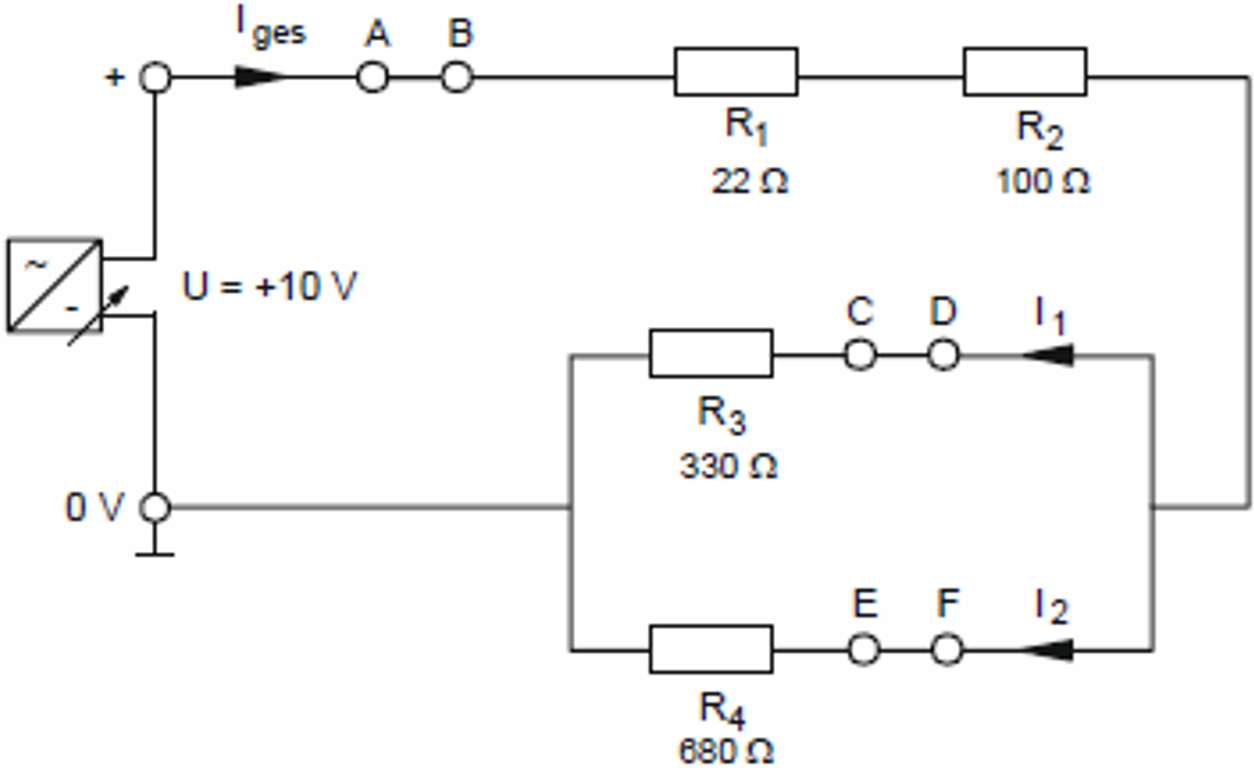
\includegraphics[width=0.6\textwidth]{Pictures/Kapitel3/Mischen von Reihen und Parallelschaltung.png}
    \caption{Schaltung zur Untersuchung des Stromflusses}
    \label{fig:K3A1}
\end{figure}

\subsection{Versuchsdurchführung}
Die Durchführung erfolgt in folgenden Schritten:
\begin{enumerate}
    \item Aufbau der Schaltung gemäß Abbildung~\ref{fig:K3A1}.
    \item Überprüfung der Versorgungsspannung \(U = 10 \, \unit{V}\) mit einem Multimeter.
    \item Messung der Teilströme an den Punkten A-B (\(I_{ges}\)), C-D (\(I_1\)) und E-F (\(I_2\)).
    \item Erfassung der Spannungen an den Widerständen \(R_1\), \(R_2\), \(R_3\) und \(R_4\).
    \item Vergleich der Messwerte mit den theoretischen Berechnungen.
\end{enumerate}

\subsection{Ergebnisse}
Die gemessenen und berechneten Werte sind in Tabelle~\ref{tab:K3T1} und Tabelle~\ref{tab:K3T2} zusammengefasst. Die theoretischen Werte werden mit den folgenden Gleichungen berechnet: 
\begin{align*}
    R_{ges} &= R_1 + R_2 + \frac{R_3 \cdot R_4}{R_3 + R_4}\\
    I_{ges} &= \frac{U}{R_{ges}}\\
    I_1 &= I_{ges} \cdot \frac{R_4}{R_3 + R_4}\\
    I_2 &= I_{ges} \cdot \frac{R_3}{R_3 + R_4}
\end{align*}

\begin{table}[H]
    \centering
    \caption{Gemessene und berechnete Ströme}
    \begin{tabular}{c c c c}
        \hline
        \multicolumn{4}{c}{Teilströme und Gesamtstrom/\unit{mA}}\\
        \hline
        \multicolumn{4}{c}{Messpunkte}\\
        \hline
       & A-B ($I_{ges}$) & C-D ($I_1$) & E-F ($I_2$)\\
        gemessen & 29,08 & 19,67 & 9,43\\
        berechnet & 29,05 & 19,56 & 9,49\\
        \hline     
    \end{tabular}
    \label{tab:K3T1}
\end{table}

\begin{table}[H]
    \centering
    \caption{Gemessene und berechnete Spannungen}
    \begin{tabular}{c c c c c}
         \hline 
         \multicolumn{5}{c}{Teilspannungen/\unit{V}} \\
         \hline
        & $U_{R1}$ & $U_{R2}$ & $U_{R3}$ & $U_{R4}$\\
        gemessen & 0,63 & 2,63 & 6,41 & 6,41\\
        berechnet & 0,64 & 2,90 & 6,50 & 6,50\\
         \hline
    \end{tabular}
    \label{tab:K3T2}
\end{table}

\subsection{Diskussion und Interpretation}
Die Messergebnisse stimmen gut mit den theoretischen Berechnungen überein. Kleine Abweichungen sind auf Messfehler oder Toleranzen der Widerstände zurückzuführen. Die Teilströme \(I_1\) und \(I_2\) folgen den Erwartungen der Stromteilerregel, während die gemessenen Spannungen die Eigenschaften der Reihen- und Parallelschaltungen bestätigen. Besonders hervorzuheben ist die hohe Übereinstimmung der Gesamtstrommessung \(I_{ges}\).

\paragraph{Abweichungen:}
\begin{itemize}
    \item \textbf{Widerstandstoleranzen:} Kleine Abweichungen in den nominellen Widerstandswerten könnten die Ergebnisse beeinflusst haben.
    \item \textbf{Messgeräte:} Die Genauigkeit der Multimeter beeinflusst die Messwerte geringfügig.
\end{itemize}

\newpage
\section{Unbelasteter Spannungsteiler} \label{c: Kapitel4}
Ein Spannungsteiler ist eine grundlegende Schaltung in der Elektrotechnik, die verwendet wird, um eine Eingangsspannung $U_{in}$ in eine proportionale Ausgangsspannung $U_{out}$ zu unterteilen. Dies wird durch die gezielte Auswahl und Dimensionierung zweier in Reihe geschalteter Widerstände $R_1$ und $R_2$ erreicht.

Die Ausgangsspannung wird dabei durch das Verhältnis der Widerstandswerte bestimmt und kann mit der folgenden Gleichung berechnet werden:
\begin{align} \label{eq:Spannungsteiler}
   U_{out} &= U_{in} \cdot \frac{R_2}{R_1 + R_2} = U_{in} \cdot k
\end{align}
In dieser Gleichung beschreibt der Faktor $k$ den Teilungsfaktor, der bestimmt, welcher Anteil der Eingangsspannung am Widerstand $R_2$ abfällt. Der Spannungsteiler ist ideal für Anwendungen, bei denen eine reduzierte Spannung benötigt wird, z. B. zur Anpassung eines Signals an einen bestimmten Eingangswert.

Ein wichtiger Aspekt eines unbelasteten Spannungsteilers ist, dass keine zusätzliche Last am Ausgang $U_{out}$ angeschlossen ist. Dadurch bleibt der Spannungsabfall ausschließlich durch die Widerstände $R_1$ und $R_2$ definiert. Sobald jedoch eine Last angeschlossen wird, verändert sich die Ausgangsspannung aufgrund des zusätzlichen Stroms, der durch die Last fließt.

Um diesen Zusammenhang besser zu verstehen, wird eine Schaltung gemäß Abbildung~\ref{fig:K4A1} aufgebaut. In dieser Schaltung werden die Spannungen $U_1$ und $U_2$ gemessen. Die gemessenen Werte werden anschließend in Tabelle \ref{tab:K4T1} dokumentiert und grafisch in Form von Kennlinien dargestellt (siehe Abbildung \ref{fig:K4A2}).
\vspace{0.5cm}
\begin{figure}[H]
    \centering
    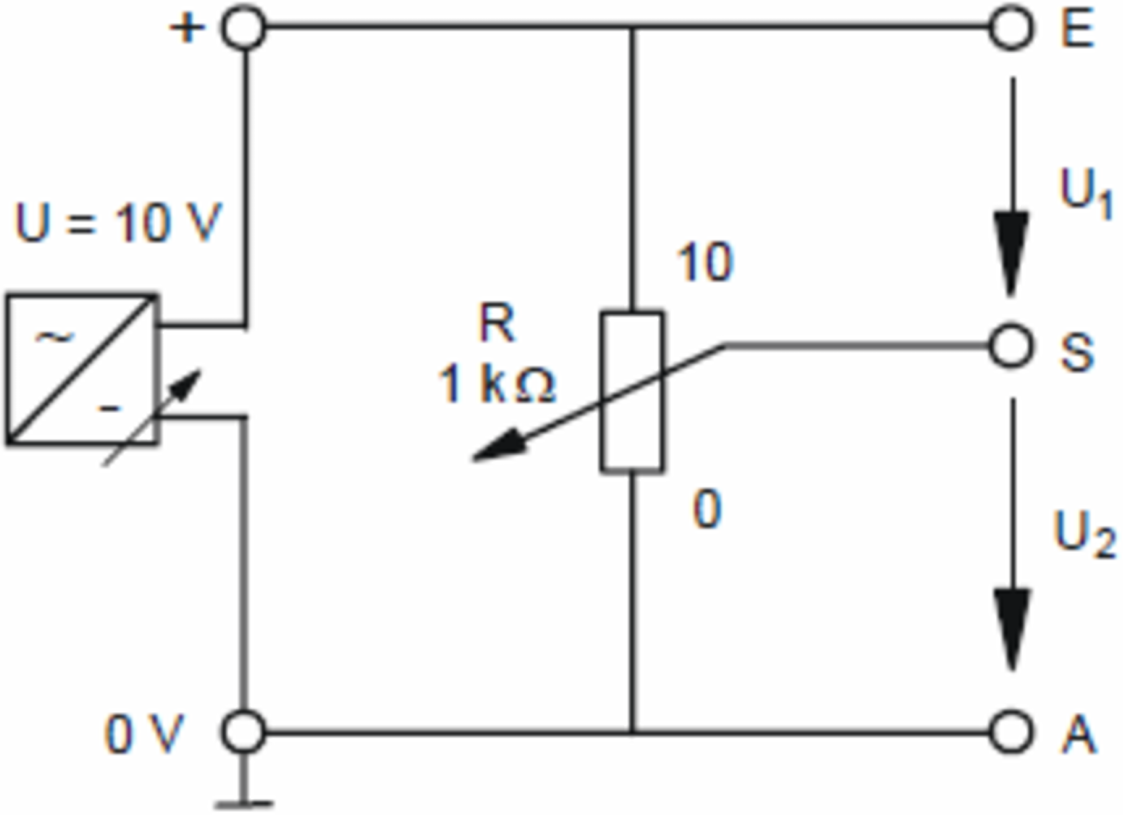
\includegraphics[width=0.5\textwidth]{Pictures/Kapitel4/Unbelasteter Spannungsteiler.png}
    \caption{Schematischer Aufbau unbelasteter Spannungsteiler}
    \label{fig:K4A1}
\end{figure}

\subsection{Messwerte}

Die Potentiometerstellung $\alpha$ gibt an, wie der Gesamtwiderstand $R$ auf die beiden Teilwiderstände $R_1$ und $R_2$ aufgeteilt wird. Ein hoher $\alpha$-Wert führt zu größeren Widerstanden von $R_2$ und kleineren von $R_1$, wodurch die Ausgangsspannung $U_2$ ansteigt.

\begin{table}[H]
\centering
\caption{Spannung $U$ bei Potentiometerstellung $\alpha$}
\begin{tabular}{ c c c c c c c c c c c c} % Abstand der Spalten
\toprule
    $\alpha$ & 0 & 1 & 2 & 3 & 4 & 5 & 6 & 7 & 8 & 9 & 10 \\
     \midrule
    $U_1/\,\unit{V}$ & 10,00 & 9,42 & 7,98 & 6,90 & 5,74 & 4,70 & 3,58 & 2,62 & 1,59 & 0,55 & 0,00 \\
    $U_2/\,\unit{V}$ & 0,00 & 0,58 & 2,02 & 3,09 & 4,24 & 5,28 & 6,39 & 7,35 & 8,38 & 9,42 & 10,00 \\
    \bottomrule
\end{tabular}
\label{tab:K4T1}%Rechnerische Tabelle2
\end{table}
\vspace{0.5cm}
\begin{figure}[H]
\centering
\begin{tikzpicture}
\begin{axis}[
    width=0.6\textwidth,
    xlabel={Potentiometerstellung $\alpha$},
    ylabel={Spannung $U/\,\unit{V}$},
    grid=major,
    legend style={at={(0.5,0.9)}, anchor=north, font=\scriptsize},
    xtick={0,1,2,3,4,5,6,7,8,9,10},
    xticklabels={0,1,2,3,4,5,6,7,8,9,10},
    ytick={0,2,4,6,8,10},
    font=\footnotesize
]

% Kennlinie U1
\addplot[mark=*,black] coordinates {
    (0,10.00) (1,9.42) (2,7.98) (3,6.90) (4,5.74) (5,4.70) (6,3.58) (7,2.62) (8,1.59) (9,0.55) (10,0.00)};
\addlegendentry{$U_1$}

% Kennlinie U2
\addplot[mark=square*,gray] coordinates {
    (0,0.00) (1,0.58) (2,2.02) (3,3.09) (4,4.24) (5,5.28) (6,6.39) (7,7.35) (8,8.38) (9,9.42) (10,10.00)};
\addlegendentry{$U_2$}

\end{axis}
\end{tikzpicture}
\caption{Kennlinie $U_1 =f(\alpha)$ und $U_2 =f(\alpha)$}
\label{fig:K4A2}
\end{figure}

Die berechneten Werte stimmen gut mit den gemessenen Spannungen überein. Abweichungen können auf Rundungsfehler oder geringe Messunsicherheiten zurückzuführen sein.

\newpage

\subsection{Rechnerische Überprüfung}

Die Messwerte aus Tabelle \ref{tab:K4T1} werden anhand der Gleichung~\eqref{eq:Spannungsteiler} überprüft. Die Ausgangsspannungen $U_1$ und $U_2$ hängen vom Verhältnis der Widerstände $R_1$ und $R_2$ ab. Für einen Gesamtwiderstand $R = 1\,\mathrm{k\Omega}$ und eine Eingangsspannung $U_{in} = 10\,\mathrm{V}$ gilt:

\[
U_1 = U_{in} \cdot \frac{R_1}{R_1 + R_2}, \quad U_2 = U_{in} \cdot \frac{R_2}{R_1 + R_2}
\]

Die Potentiometerstellung $\alpha$ bestimmt das Verhältnis von $R_1$ und $R_2$. Bei einer linearen Verteilung des Potentiometers gilt:

\begin{equation}
    R_1 = R \cdot \frac{\alpha}{10}
\end{equation}
\begin{equation}
    \quad R_2 = R \cdot \left( 1 - \frac{\alpha}{10} \right)
\end{equation}

Durch Einsetzen in die Spannungsteilerformel ergeben sich die berechneten Werte für $U_1$ und $U_2$, wie in Tabelle \ref{tab:K4T2} dargestellt:

\begin{table}[H]
\centering
\caption{Rechnerisch ermittelte Spannungen $U_1$ und $U_2$ bei Potentiometerstellung $\alpha$}
\begin{tabular}{c c c c c c c c c c c c}
\toprule
$\alpha$ & 0 & 1 & 2 & 3 & 4 & 5 & 6 & 7 & 8 & 9 & 10 \\
\midrule
$U_1/\,\unit{V}$ & 10,00 & 9,00 & 8,00 & 7,00 & 6,00 & 5,00 & 4,00 & 3,00 & 2,00 & 1,00 & 0,00 \\
$U_2/\,\unit{V}$ & 0,00 & 1,00 & 2,00 & 3,00 & 4,00 & 5,00 & 6,00 & 7,00 & 8,00 & 9,00 & 10,00 \\
\bottomrule
\end{tabular}
\label{tab:K4T2}
\end{table}

\newpage

\section{Belasteter Spannungsteiler}

\subsection{Einleitung}
Ein belasteter Spannungsteiler wird verwendet, um eine bestimmte Ausgangsspannung zu erzeugen, selbst wenn ein Verbraucher angeschlossen ist. Im Vergleich zum unbelasteten Spannungsteiler (siehe Kapitel \ref{c: Kapitel4} ) wird hierbei die Belastung durch einen weiteren Widerstand berücksichtigt (siehe Abbildung \ref{fig:K5A1}), der parallel zum Teilwiderstand geschaltet ist.

\vspace{0.5cm}
\begin{figure}[H]
    \centering
    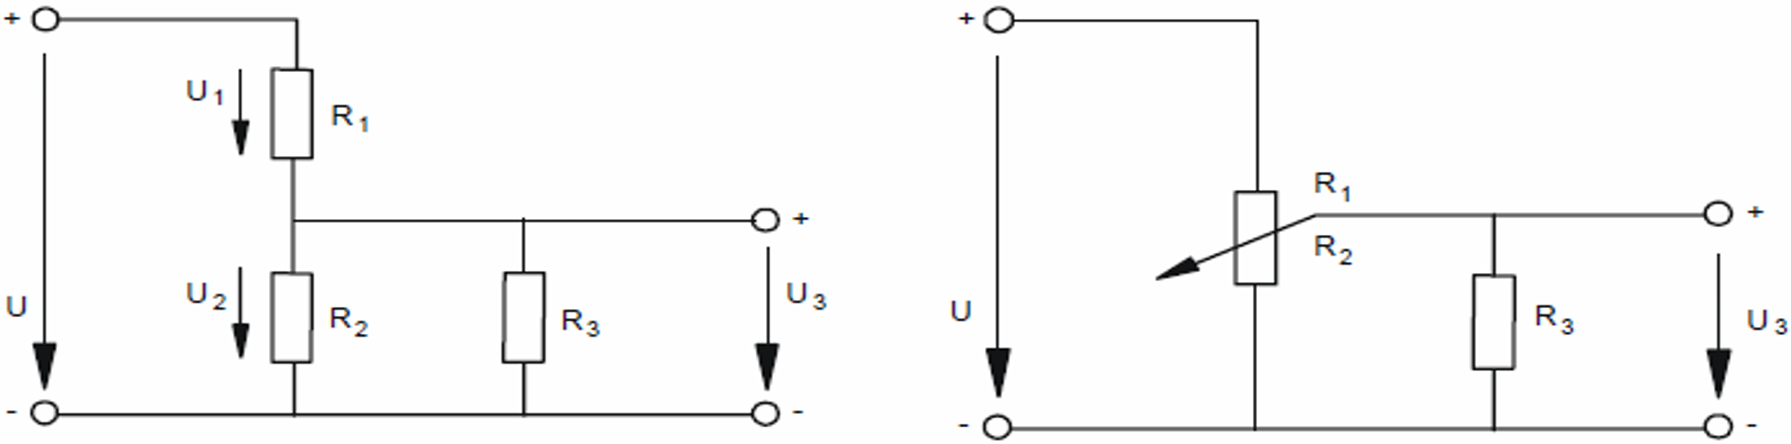
\includegraphics[width=0.8\linewidth]{Pictures/Kapitel5/Belasteter Spannungsteiler 2.png}
    \caption{Belasteter Spannungsteiler}
    \label{fig:K5A1}
\end{figure}

Ein Spannungsteiler besteht aus zwei Widerständen, die in Serie geschaltet sind. Die Ausgangsspannung $U_{out}$ wird über einem der Widerstände abgegriffen. Sobald ein Verbraucher mit Widerstand $R_L$ an die Ausgangsklemmen angeschlossen wird, verändert sich die effektive Last des Spannungsteilers. Die Ausgangsspannung lässt sich nun mithilfe der Ersatzwiderstände berechnen:
\begin{equation} \label{eq:Spannungsteiler2}
    U = U_3 \cdot \frac{R_2 \parallel R_3}{R_1 + (R_2 \parallel R_3)}
\end{equation}
wobei $R_2 \parallel R_3$ der Ersatzwiderstand des parallelen Zweigs ist:
\begin{equation} \label{eq:Parallelschaltung2}
    R_2 \parallel R_3 = \frac{R_2 \cdot R_3}{R_2 + R_3}
\end{equation}

\subsection{Versuchsaufbau}
Für den Versuch wird die in Abbildung~\ref{fig:K5A2} dargestellte Schaltung aufgebaut. Die Eingangsspannung $U_{in}$ beträgt $5\,\unit{V}$, und der Spannungsteiler wird mit einem variablen Widerstand $R = 1\,\unit{\kohm}$ (Potentiometer) realisiert. Zusätzlich wird ein Verbraucherwiderstand $R_3$ parallel zum unteren Teil des Potentiometers geschaltet.

\begin{figure}[H]
    \centering
    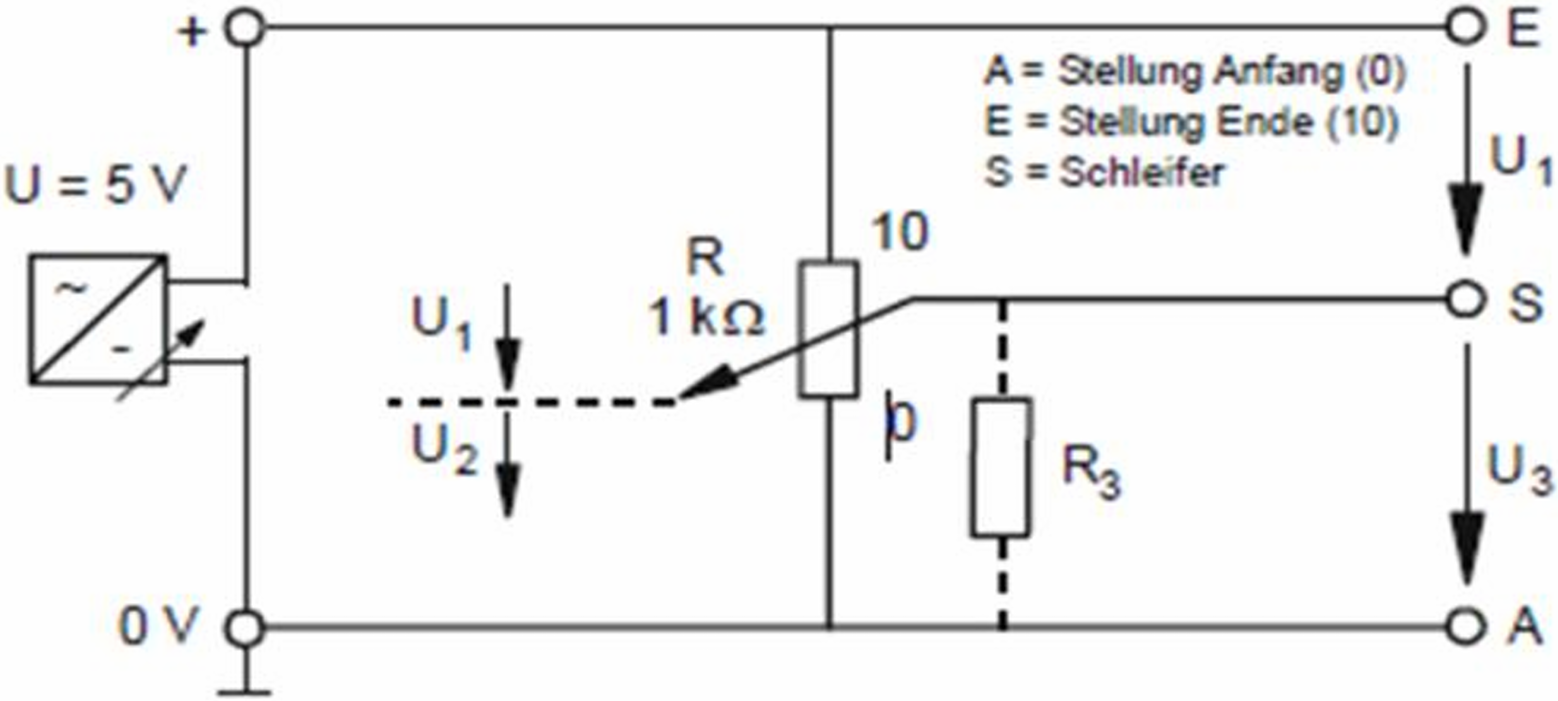
\includegraphics[width=0.6\textwidth]{Pictures/Kapitel5/Belasteter Spannungsteiler.png}
    \caption{Schematischer Aufbau des belasteten Spannungsteilers}
    \label{fig:K5A2}
\end{figure}

\subsection{Versuchsdurchführung}

\begin{enumerate}
    \item Der Spannungsteiler wird so eingestellt, dass die Ausgangsspannung $U_3$ variiert werden kann.
    \item Für jede Einstellung des Potentiometers wird die Spannungen $U_3$ gemessen.
    \item Die Messwerte werden in Tabelle~\ref{tab:K5T1} dokumentiert, grafisch in Form einer Kennlinie in Abbildung~\ref{fig:K5A3} dargestellt und anschließend mit den theoretisch berechneten Werten (siehe Tabelle~\ref{tab:K5T2}) verglichen.
\end{enumerate}

\subsection{Ergebnisse}

Die Messergebnisse des belasteten Spannungsteilers sind in Tabelle~\ref{tab:K5T1} dargestellt:

\begin{table}[H]
\centering
\begin{footnotesize}
\caption{Messwerte des belasteten Spannungsteilers bei Potentiometerstellung $\alpha$.}
\begin{tabular}{c c c c c c c c c c c c}
\toprule
$\alpha$ & 0 & 1 & 2 & 3 & 4 & 5 & 6 & 7 & 8 & 9 & 10 \\
\midrule
$U_3/\,\unit{V}$ $R_3=100\,\unit{\ohm}$ & 0,00 & 0,18 & 0,34 & 0,47 & 0,59 & 0,72 & 0,90 & 1,17 & 1,73 & 2,75 & 4,91\\
$U_3/\,\unit{V}$ $R_3=470\,\unit{\ohm}$& 0,00 & 0,26 & 0,64 & 1,03 & 1,36 & 1,66 & 2,06 & 2,50 & 3,21 & 4,06&4,93 \\
$U_3/\,\unit{V}$ $R_3=1\,\unit{\kohm}$ & 0,00 & 0,27 & 0,73 & 1,23 & 1,67 & 2,04 & 2,50 & 2,97 & 3,64 & 4,32 &4,94 \\
\bottomrule
\end{tabular}
\label{tab:K5T1}
\end{footnotesize}
\end{table}

Die gemessenen Werte stimmen gut mit den berechneten Werten (siehe Tabelle~\ref{tab:K5T2}) überein. Abweichungen sind insbesondere in den unteren Potentiometerstellungen erkennbar, was auf systematische Messfehler oder Widerstandstoleranzen zurückzuführen sein könnte.

\begin{figure}[H]
\centering
\begin{tikzpicture}
\begin{axis}[
    width=0.6\textwidth,
    xlabel={Potentiometerstellung $\alpha$},
    ylabel={Spannung $U_3/\,\unit{V}$},
    grid=major,
    legend style={at={(0.1,0.9)}, anchor=north west, font=\scriptsize},
    xtick={0,1,2,3,4,5,6,7,8,9,10},
    ytick={0,1,2,3,4,5},
    font=\footnotesize
]

% Daten für R3 = 100 Ohm
\addplot[mark=*,black] coordinates {
    (0,0.00) (1,0.18) (2,0.34) (3,0.47) (4,0.59) (5,0.72) (6,0.90) (7,1.17) (8,1.73) (9,2.75) (10,4.91)};
\addlegendentry{$R_3 = 100\,\unit{\ohm}$}

% Daten für R3 = 470 Ohm
\addplot[mark=square*,black,dashed] coordinates {
    (0,0.00) (1,0.26) (2,0.64) (3,1.03) (4,1.36) (5,1.66) (6,2.06) (7,2.50) (8,3.21) (9,4.06) (10,4.93)};
\addlegendentry{$R_3 = 470\,\unit{\ohm}$}

% Daten für R3 = 1 kOhm
\addplot[mark=triangle*,black,dotted] coordinates {
    (0,0.00) (1,0.27) (2,0.73) (3,1.23) (4,1.67) (5,2.04) (6,2.50) (7,2.97) (8,3.64) (9,4.32) (10,4.94)};
\addlegendentry{$R_3 = 1\,\unit{\kohm}$}

\end{axis}
\end{tikzpicture}
\caption{Kennlinie $U_3 = f(\alpha)$ bei konstanter Eingangsspannung}
\label{fig:K5A3}
\end{figure}

\subsection{Rechnerische Überprüfung}
Die Messwerte werden mit der Gleichung \eqref{eq:Spannungsteiler2} überprüft. Die berechneten Werte sind in Tabelle~\ref{tab:K5T2} dargestellt:

\begin{table}[H]
\centering
\begin{footnotesize}
\caption{Rechnerische Überprüfung der Messwerte des belasteten Spannungsteilers}
\begin{tabular}{c c c c c c c c c c c c }
\toprule
$\alpha$ & 0 & 1 & 2 & 3 & 4 & 5 & 6 & 7 & 8 & 9 & 10 \\
\midrule
$U_3/\,\unit{V}$ $R_3=100\,\unit{\ohm}$ & 0,0 & 0,26 & 0,38 & 0,48 & 0,59 & 0,71 & 0,88 & 1,13 & 1,54 & 2,37 & 5,0 \\
$U_3/\,\unit{V}$ $R_3=470\,\unit{\ohm}$ & 0,0 & 0,42 & 0,75 & 1,04 & 1,32 & 1,63 & 1,99 & 2,42 & 2,98 & 3,78 & 5,0 \\
$U_3/\,\unit{V}$ $R_3=1\,\unit{\kohm}$ & 0,0 & 0,46 & 0,86 & 1,24 & 1,61 & 2,0 & 2,42 & 2,89 & 3,45 & 4,13 & 5,0 \\
\bottomrule
\end{tabular}
\label{tab:K5T2}
\end{footnotesize}
\end{table}

\begin{figure}[H]
\centering
\begin{tikzpicture}
\begin{axis}[
    width=0.55\textwidth,
    xlabel={Potentiometerstellung $\alpha$},
    ylabel={Spannung $U_3/\,\unit{V}$},
    grid=major,
    legend style={at={(0.1,0.9)}, anchor=north west, font=\scriptsize},
    xtick={0,1,2,3,4,5,6,7,8,9,10},
    ytick={0,1,2,3,4,5},
    font=\footnotesize
]

% Daten für R3 = 100 Ohm (aktualisierte Werte)
\addplot[mark=*,black] coordinates {
    (0,0.0) (1,0.26) (2,0.38) (3,0.48) (4,0.59) (5,0.71) (6,0.88) (7,1.13) (8,1.54) (9,2.37) (10,5.0)};
\addlegendentry{$R_3 = 100\,\unit{\ohm}$}

% Daten für R3 = 470 Ohm (aktualisierte Werte)
\addplot[mark=square*,black,dashed] coordinates {
    (0,0.0) (1,0.42) (2,0.75) (3,1.04) (4,1.32) (5,1.63) (6,1.99) (7,2.42) (8,2.98) (9,3.78) (10,5.0)};
\addlegendentry{$R_3 = 470\,\unit{\ohm}$}

% Daten für R3 = 1 kOhm (aktualisierte Werte)
\addplot[mark=triangle*,black,dotted] coordinates {
    (0,0.0) (1,0.46) (2,0.86) (3,1.24) (4,1.61) (5,2.0) (6,2.42) (7,2.89) (8,3.45) (9,4.13) (10,5.0)};
\addlegendentry{$R_3 = 1\,\unit{\kohm}$}

\end{axis}
\end{tikzpicture}
\caption{Kennlinie der theoretischen Werte $U_3 = f(\alpha)$ bei konstanter Eingangsspannung.}
\label{fig:K5A4}
\end{figure}


\subsection{Diskussion und Interpretation}
Die Ergebnisse verdeutlichen den Einfluss des parallel geschalteten Verbraucherwiderstands $R_3$ auf die Ausgangsspannung $U_3$ des Spannungsteilers. Im Vergleich zum unbelasteten Fall, bei dem der Spannungsteiler nur aus den Widerständen $R_1$ und $R_2$ besteht, führt die zusätzliche Belastung durch $R_3$ zu einer Verringerung der effektiven Ausgangsspannung. Diese Verringerung ist umso ausgeprägter, je kleiner der Wert von $R_3$ ist. 

Die theoretischen Werte zeigen, dass bei \(R_3 = 100\,\unit{\ohm}\) die Belastung deutlich stärker ausfällt als bei \(R_3 = 470\,\unit{\ohm}\) oder \(R_3 = 1\,\unit{\kohm}\). Dies liegt daran, dass der Ersatzwiderstand $R_2 \parallel R_3$ mit sinkendem $R_3$ ebenfalls sinkt, was den Spannungsabfall am oberen Widerstand $R_1$ erhöht und die Ausgangsspannung verringert.

Darüber hinaus wird festgestellt, dass die Abweichungen zwischen den gemessenen und theoretischen Werten in den niedrigen Potentiometerstellungen (\(\alpha \leq 4\)) am größten sind. Diese Abweichungen können durch folgende Faktoren erklärt werden:
\begin{itemize}
    \item Kontaktwiderstände: An den Anschlüssen des Potentiometers können zusätzliche Widerstände auftreten, die den Gesamtwiderstand beeinflussen.
    \item Toleranzen der Widerstände: Kommerzielle Widerstände haben typischerweise eine Toleranz von 1\% bis 5\%, die die Ergebnisse insbesondere bei kleinen Widerstandswerten stark beeinflussen können.
    \item Messgeräteungenauigkeiten: Die Genauigkeit der verwendeten Multimeter und deren Kalibrierung spielen eine wichtige Rolle, insbesondere bei niedrigen Spannungen.
    \item Systematische Fehler: Der Aufbau der Schaltung kann zusätzliche Verluste verursachen, beispielsweise durch Leitungswiderstände oder nicht ideale Kontakte.
\end{itemize}

Eine interessante Beobachtung ist die Nichtlinearität des Spannungsverlaufs bei hohen Potentiometerstellungen (\(\alpha > 7\)). In diesem Bereich wird $R_2$ dominant, und der Ersatzwiderstand $R_2 \parallel R_3$ nähert sich dem Wert von $R_3$. Dadurch wird der Spannungsabfall am Verbraucher geringer, was zu einem flacheren Anstieg der Kennlinie führt.

Der belastete Spannungsteiler findet breite Anwendung in der Elektronik, insbesondere bei Spannungsteilerregelungen und Signalabschaltungen. Das Verständnis der Belastung ist entscheidend, um eine korrekte Dimensionierung der Widerstände und Verbraucher sicherzustellen. Ein häufiges Beispiel ist die Anpassung von Spannungssignalen an analoge oder digitale Eingänge, bei denen die Eingangsimpendanz des Folgeschaltkreises als Verbraucher wirkt.

Um die Auswirkungen der Belastung weiter zu untersuchen und die Ergebnisse zu optimieren, könnten folgende Maßnahmen durchgeführt werden:
\begin{itemize}
    \item Einsatz präziser Widerstände: Verwendung von Widerständen mit geringere Toleranzen, beispielsweise 0,1\%.
    \item Vermeidung von Kontaktwiderständen: Verwendung hochwertiger Kontaktstellen und feste Lötverbindungen anstelle von Steckverbindern.
    \item Erhöhung der Eingangsspannung: Dies würde die Messung bei niedrigen Spannungen präziser machen, da relative Fehler reduziert werden.
\end{itemize}

Zusammenfassend zeigt der Versuch die Bedeutung einer genauen Analyse von belasteten Spannungsteilern in der Elektrotechnik. Die Erkenntnisse sind von grundlegender Bedeutung für die Dimensionierung und Optimierung elektronischer Schaltungen.


\newpage
\section{Spannungs- und Strommessung}
\subsection{Einleitung}
Die Messung von Spannung und Strom ist eine grundlegende Aufgabe in der Elektrotechnik. Je nach Art des Verbrauchers (hochohmig oder niederohmig) hat die Wahl der Messmethode - spannungsrichtig oder stromrichtig - einen wesentlichen Einfluss auf die Genauigkeit der Messergebnisse. Die beiden Methoden unterscheiden sich in der Art, wie Strom- und Spannungsmesser in die Schaltung eingebunden werden. Ziel dieses Versuchs ist es, die Unterschiede beider Methoden zu untersuchen und die resultierenden Widerstandswerte für verschiedene Verbraucher zu vergleichen.

\subsection{Theoretische Grundlagen}
\paragraph{Spannungsrichtige Messung}
Bei der spannungsrichtigen Messung wird der Strommesser in Reihe und der Spannungsmesser parallel zum Verbraucher geschaltet. Diese Methode ist besonders geeignet für niederohmige Verbraucher, da der Einfluss des Parallelwiderstands des Spannungsmessers vernachlässigbar ist (siehe Abbildung~\ref{subfig:K6A1a}).

\paragraph{Stromrichtige Messung}
Im Gegensatz dazu wird bei der stromrichtigen Messung der Spannungsmesser parallel zum Verbraucher und Strommesser geschaltet. Diese Methode ist ideal für hochohmige Verbraucher, da der Spannungsmesser den Stromfluss kaum beeinflusst (siehe Abbildung~\ref{subfig:K6A1b}).

\subsection{Versuchsaufbau}
Für den Versuch werden zwei unterschiedliche Verbraucherwiderstände \( R \) von \( 10\,\unit{\ohm} \) (niederohmig) und \( 1\,\unit{M\ohm} \) (hochohmig) verwendet. Die Eingangsspannung beträgt konstant \( 5\,\unit{V} \). Zwei unterschiedliche Schaltungen werden aufgebaut:
\begin{itemize}
    \item \textbf{Spannungsrichtige Messung:} Nach Abbildung~\ref{subfig:K6A1a}.
    \item \textbf{Stromrichtige Messung:} Nach Abbildung~\ref{subfig:K6A1b}.
\end{itemize}
Bei beiden Methoden werden die Spannung \( U \) und der Strom \( I \) gemessen, und der Widerstand \( R \) wird mit der Gleichung \eqref{eq:Ohm'sche Gleichung} ermittelt.

\begin{figure}[H]
    \begin{subfigure}[c]{0.5\textwidth}
        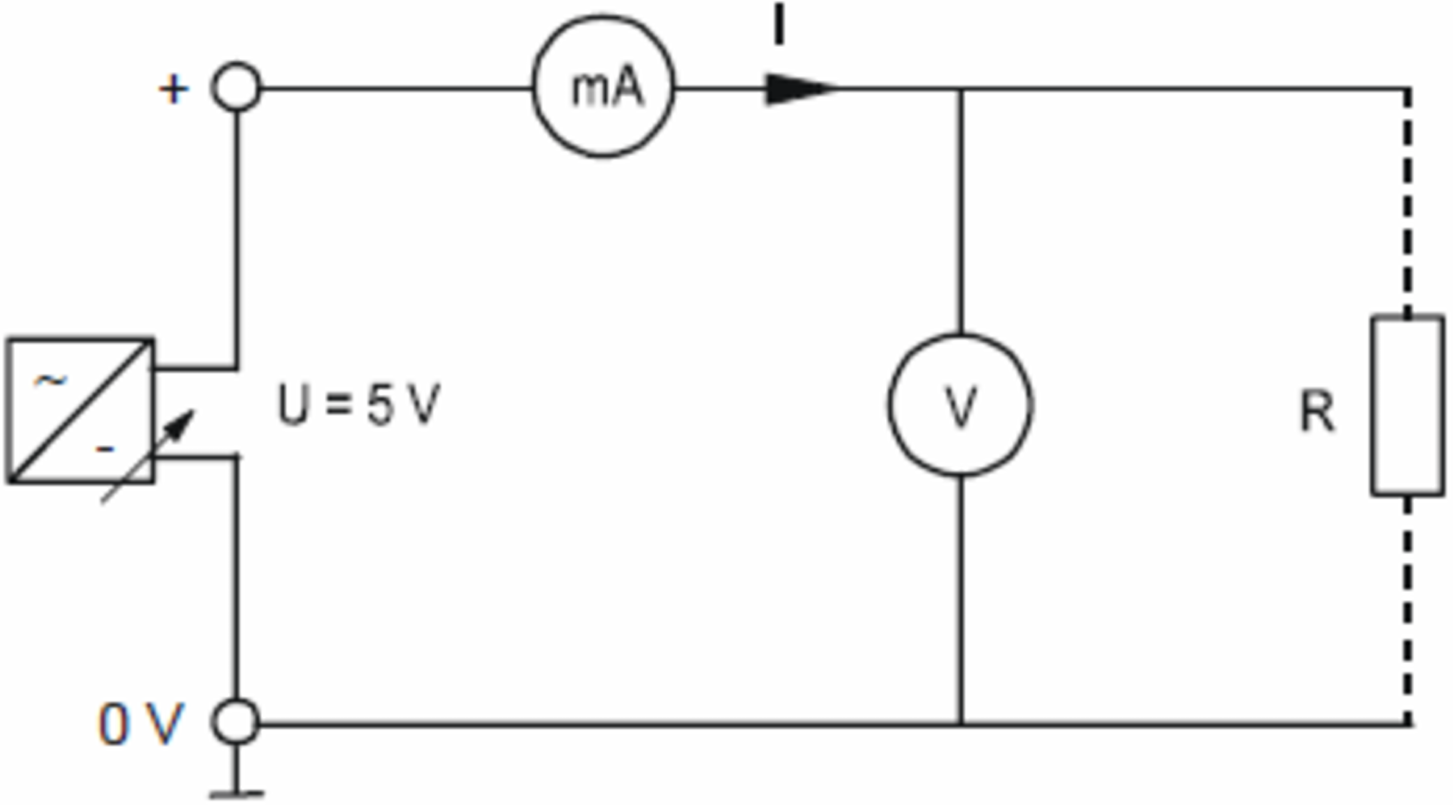
\includegraphics[width=0.95\textwidth]{Pictures/Kapitel6/Spannungsrichtig.png}
        \subcaption{Spannungsrichtige Messschaltung}
        \label{subfig:K6A1a}
    \end{subfigure}
    \begin{subfigure}[c]{0.5\textwidth}
        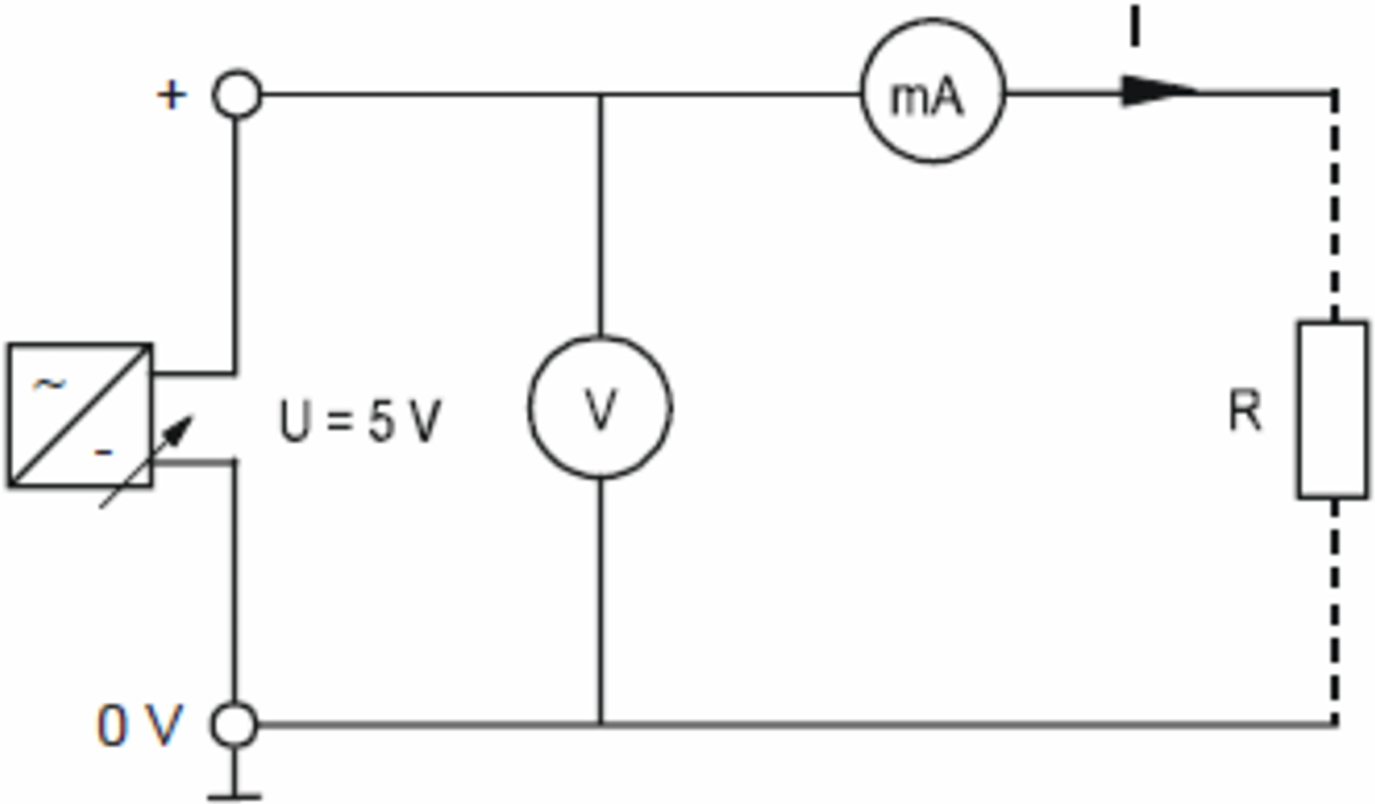
\includegraphics[width=0.9\textwidth]{Pictures/Kapitel6/Stromrichtig.png}
        \subcaption{Stromrichtige Messchaltung}
        \label{subfig:K6A1b}
    \end{subfigure}
\caption{Spannungs- und Stromrichtige Messung}
\label{fig:K6A1}
\end{figure}

\subsection{Ergebnisse}
Die Messwerte sind in den Tabellen~\ref{tab:K6T1} und~\ref{tab:K6T2} dargestellt. Sie zeigen die gemessenen und berechneten Widerstandswerte für beide Methoden.

\begin{table}[H]
\centering
\begin{footnotesize}
\caption{Ergebnisse der spannungsrichtigen Messung}
\begin{tabular}{c c c c}
\toprule
$R/\,\unit{\ohm}$ gemessen & $I/\,\unit{mA}$ & $U/\,\unit{V}$ & $R/\,\unit{\ohm}$ errechnet \\
\midrule
9,40 & 481,00 & 4,78 & 9,94 \\
\(1,0020\cdot10^6\) & 0,0054 & 4,9800 & \(0,9220 \cdot 10^6\) \\
\bottomrule
\end{tabular}
\label{tab:K6T1}
\end{footnotesize}
\end{table}

\begin{table}[H]
\centering
\begin{footnotesize}
\caption{Ergebnisse der stromrichtigen Messung}
\begin{tabular}{c c c c}
\toprule
$R/\,\unit{\ohm}$ gemessen & $I/\,\unit{mA}$ & $U/\,\unit{V}$ & $R/\,\unit{\ohm}$ errechnet \\
\midrule
9,40 & 475,00 & 4,76& 10,02 \\
\(1,0020\cdot10^6\) & 0,0048 & 4,9600  & \(1,0300 \cdot 10^6\) \\
\bottomrule
\end{tabular}
\label{tab:K6T2}
\end{footnotesize}
\end{table}

Die Abweichungen zwischen gemessenen und berechneten Werten sind jedoch nicht nur auf die Wahl der Messmethode zurückzuführen, sondern auch auf folgende Faktoren, wie Messfehler, Messungenauigkeit, Toleranz usw.

\newpage
\subsection{Diskussion und Interpretation}
Die Ergebnisse zeigen, dass die Wahl der Messmethode einen signifikanten Einfluss auf die Messgenauigkeit hat:
\begin{itemize}
    \item Spannungsrichtige Messung: Diese Methode liefert bei niederohmigen Verbrauchern zuverlässige Ergebnisse, da der Spannungsmesser den Stromfluss nicht wesentlich beeinflusst. Bei hochohmigen Verbrauchern treten jedoch deutliche Abweichungen auf, da der Spannungsmesser parallel zum hohen Widerstand eine merkliche Strombelastung erzeugt.
    \item Stromrichtige Messung: Diese Methode ist ideal für hochohmige Verbraucher, da der Strommesser den Spannungsabfall nicht signifikant beeinflusst. Bei niederohmigen Verbrauchern führt der interne Widerstand des Strommessers jedoch zu einer merklichen Spannungsreduktion.
\end{itemize}

Die richtige Wahl der Messmethode ist entscheidend für exakte Ergebnisse. Während die spannungsrichtige Messung für niederohmige Verbraucher geeignet ist, sollte bei hochohmigen Verbrauchern die stromrichtige Messung angewandt werden. Dieser Versuch verdeutlicht die praktischen Auswirkungen der Messmethoden und deren Relevanz in der Elektrotechnik.

\newpage

% --- Verzeichnisse ---
\newpage
\pagenumbering{Roman} % Zurück zu römischer Nummerierung
\setcounter{page}{3} % Setzt die Nummerierung auf III

\listoffigures % Abbildungsverzeichnis
\addcontentsline{toc}{section}{Abbildungsverzeichnis} % Hinzufügen ins Inhaltsverzeichnis
\newpage

\listoftables % Tabellenverzeichnis
\addcontentsline{toc}{section}{Tabellenverzeichnis} % Hinzufügen ins Inhaltsverzeichnis
\newpage

% --- Literaturverzeichnis ---
\nocite{*} % Zitieren aller Einträge, auch wenn nicht im Text referenziert
\bibliography{Sources} % Literaturverzeichnis
\addcontentsline{toc}{section}{Literaturverzeichnis} % Hinzufügen ins Inhaltsverzeichnis
\newpage

\begin{appendix}
	\section{Berechnungen}\label{appA}

\large \textbf{Abschnitt 2: Ohmsches Gesetz}

Tabelle \ref{tab:K2T3}:
\begin{align*}
    I &= \frac{U}{R}=\frac{\SI{2}{V}}{\SI{100}{\Omega}}=\SI{0,02}{mA}=\SI{20}{mA}\\
    I &= \frac{U}{R}=\frac{\SI{2}{V}}{\SI{300}{\Omega}}=\SI{0,00667}{mA}=\SI{6,67}{mA}
\end{align*}
Tabelle \ref{tab:K2T4}:
\begin{align*}
    I &= \frac{U}{R}=\frac{\SI{12}{V}}{\SI{100}{\Omega}}=\SI{0,12}{mA}=\SI{120}{mA}\\
    I &= \frac{U}{R}=\frac{\SI{8}{V}}{\SI{100}{\Omega}}=\SI{0,08}{mA}=\SI{80}{mA}\\
    I &= \frac{U}{R}=\frac{\SI{4}{V}}{\SI{100}{\Omega}}=\SI{0,04}{mA}=\SI{40}{mA}
\end{align*}

\large \textbf{Abschnitt 3: Mischen von Serien- und Parallelschaltungen}

Tabelle \ref{tab:K3T1}:
\begin{align*}
    R_{\text{ges}} &= R_1 + R_2 + \frac{R_3 \cdot R_4}{R_3 + R_4} = 22 \, \Omega + 100 \, \Omega + \frac{680 \, \Omega \cdot 330 \, \Omega}{680 \, \Omega + 330 \, \Omega} \\
    &= 122 \, \Omega + \frac{224400 \, \Omega^2}{1010 \, \Omega} = 122 \, \Omega + 222.18 \, \Omega = 344.18 \, \Omega
\end{align*}
\begin{align*}
    I_{\text{ges}} &= \frac{U}{R_{\text{ges}}} = \frac{10 \, \mathrm{V}}{344.18 \, \Omega} = 0.02905 \, \mathrm{A} \, =29.05 \, \mathrm{mA}
\end{align*}
\begin{align*}
    I_1 &= I_{\text{ges}} \cdot \frac{R_3}{R_3 + R_4} = 0.02905 \, \mathrm{A} \cdot \frac{680 \, \Omega}{680 \, \Omega + 330 \, \Omega} \\
    &= 0.02905 \, \mathrm{A} \cdot \frac{680 \, \Omega}{1010 \, \Omega} = 0.01956 \, \mathrm{A} \, = 19.56 \, \mathrm{mA}
\end{align*}
\begin{align*}
    U_{R1} &= I_{\text{ges}} \cdot R_1 = 0.02905 \, \mathrm{A} \cdot 22 \, \Omega = 0.6391 \, \mathrm{V}
\end{align*}

\large \textbf{Abschnitt 4: Unbelasteter Spannungsteiler}

Tabelle \ref{tab:K3T2}:
\begin{align*}
    R_2 &= R \cdot \frac{\alpha}{10} = 1 \, \mathrm{k\Omega} \cdot \frac{1}{10} = 0.1 \, \mathrm{k\Omega} = 100 \, \Omega \\
    R_1 &= R \cdot \left( 1 - \frac{\alpha}{10} \right) = 1 \, \mathrm{k\Omega} \cdot \left( 1 - \frac{1}{10} \right) = 0.9 \, \mathrm{k\Omega} = 900 \, \Omega
\end{align*}
\begin{align*}
    U_2 &= U_{\text{in}} \cdot \frac{R_2}{R_1 + R_2} = 10 \, \mathrm{V} \cdot \frac{100 \, \Omega}{100 \, \Omega + 900 \, \Omega} = 10 \, \mathrm{V} \cdot \frac{100}{1000} = 1 \, \mathrm{V} \\
    U_1 &= U_{\text{in}} \cdot \frac{R_1}{R_1 + R_2} = 10 \, \mathrm{V} \cdot \frac{900 \, \Omega}{100 \, \Omega + 900 \, \Omega} = 10 \, \mathrm{V} \cdot \frac{900}{1000} = 9 \, \mathrm{V}
\end{align*}

\large \textbf{Abschnitt 5: Belasteter Spannungsteiler}

Tabelle \ref{tab:K4T2}:
\begin{align*}
    R_{\text{ers}} &= \frac{R_2 \cdot R_3}{R_2 + R_3} 
    = \frac{100 \, \Omega \cdot 100 \, \Omega}{100 \, \Omega + 100 \, \Omega} 
    = \frac{10000 \, \Omega^2}{200 \, \Omega} 
    = 50 \, \Omega
\end{align*}
\begin{align*}
    R_{\text{ges}} &= R_1 + R_{\text{ers}} 
    = 900 \, \Omega + 50 \, \Omega 
    = 950 \, \Omega
\end{align*}
\begin{align*}
    I_{\text{ges}} &= \frac{U_{\text{in}}}{R_{\text{ges}}} 
    = \frac{5 \, \mathrm{V}}{950 \, \Omega} 
    = 0.00526 \, \mathrm{A} \, (5.26 \, \mathrm{mA}).
\end{align*}
\begin{align*}
    U_3 &= I_{\text{ges}} \cdot R_{\text{ers}} 
    = 0.00526 \, \mathrm{A} \cdot 50 \, \Omega 
    = 0.263 \, \mathrm{V}
\end{align*}

\vspace{4cm}

\large \textbf{Abschnitt 6: Spannungs- und Strommessung}

Tabelle \ref{tab:K6T1}:
\begin{align*}
    R_{\text{errechnet}} &= \frac{U}{I} = \frac{4.78 \, \mathrm{V}}{481 \, \mathrm{mA}} = \frac{4.78 \, \mathrm{V}}{0.481 \, \mathrm{A}} = 9.94 \, \Omega
\end{align*}
\begin{align*}
    R_{\text{errechnet}} &= \frac{U}{I} = \frac{4.9800 \, \mathrm{V}}{0.0054 \, \mathrm{mA}} = \frac{4.9800 \, \mathrm{V}}{5.4 \cdot 10^{-6} \, \mathrm{A}} = 0.9220 \cdot 10^6 \, \Omega
\end{align*}

Tabelle \ref{tab:K6T2}:
\begin{align*}
    R_{\text{errechnet}} &= \frac{U}{I} = \frac{4.76 \, \mathrm{V}}{475 \, \mathrm{mA}} = \frac{4.76 \, \mathrm{V}}{0.475 \, \mathrm{A}} = 10.02 \, \Omega
\end{align*}
\begin{align*}
    R_{\text{errechnet}} &= \frac{U}{I} = \frac{4.9600 \, \mathrm{V}}{0.0048 \, \mathrm{mA}} = \frac{4.9600 \, \mathrm{V}}{4.8 \cdot 10^{-6} \, \mathrm{A}} = 1.0300 \cdot 10^6 \, \Omega
\end{align*}

\large \textbf{Abschnitt 7: Ersatzspannungsquelle}

Tabelle \ref{tab:K7T1}:
\begin{align*}
    I_K &= \frac{U_0}{R_i} = \frac{5 \, \mathrm{V}}{22 \, \Omega} = 0.2273 \, \mathrm{A} \, (227.3 \, \mathrm{mA})
\end{align*}

Tabelle \ref{tab:K7T2}:
\begin{align*}
    I_L &= \frac{U_0}{R_L + R_i} = \frac{5 \, \mathrm{V}}{100 \, \Omega + 22 \, \Omega} = \frac{5 \, \mathrm{V}}{122 \, \Omega} = 0.04098 \, \mathrm{A} = 40.98 \, \mathrm{mA}
\end{align*}
\begin{align*}
    U_L &= U_0 - I_L \cdot R_i = 5 \, \mathrm{V} - 0.04098 \, \mathrm{A} \cdot 22 \, \Omega \\
    &= 5 \, \mathrm{V} - 0.902 \, \mathrm{V} = 4.10 \, \mathrm{V}
\end{align*}

\large \textbf{Abschnitt 8: Reihenschaltung von Spannungsquellen}

Tabelle \ref{tab:K8T1}:
\begin{align*}
    U_{ges}=\rho_1-\rho_2=5\,\unit{V}-(-15\,\unit{V})=20\,\unit{V}
\end{align*}

\large \textbf{Abschnitt 9: Parallelschaltung von Spannungsquellen}

Tabelle \ref{tab:K9T1}:\\
Leerlauf:
\begin{align*}
    I_0 &= \frac{U_{01} - U_{02}}{R_{i1} + R_{i2}} = \frac{15 - 15}{100 + 100} = 0 \, \mathrm{A}
\end{align*}
Lastfall:
\begin{align*}
    I_L &= \frac{U_{01} \cdot R_{i2} + U_{02} \cdot R_{i1}}{R_{i1} \cdot R_{i2} + R_{i1} \cdot R_L + R_{i2} \cdot R_L} \\
    &= \frac{15 \cdot 100 + 15 \cdot 100}{100 \cdot 100 + 100 \cdot 1000 + 100 \cdot 1000} \\
    &= \frac{1500 + 1500}{10000 + 100000 + 100000} \\
    &= \frac{3000}{210000} \\
    &= 0.01429 \, \mathrm{A} = 14.29 \, \mathrm{mA}
\end{align*}
\begin{align*}
    U_{12} &= I_L \cdot R_L= 0.01429 \, \mathrm{A} \cdot 1000 \, \Omega = 14.29 \, \mathrm{V}
\end{align*}

Tabelle \ref{tab:K9T2}:\\
Leerlauf:
\begin{align*}
    I_0 &= \frac{U_{01} - U_{02}}{R_{i1} + R_{i2}}= \frac{15 - 10}{100 + 100}= \frac{5}{200} = 0.025 \, \mathrm{A}= 25 \, \mathrm{mA}
\end{align*}
Lastfall:
\begin{align*}
    I_L &= \frac{15 \cdot 100 + 10 \cdot 100}{100 \cdot 100 + 100 \cdot 1000 + 100 \cdot 1000} \\
    &= \frac{1500 + 1000}{10000 + 100000 + 100000} = \frac{2500}{210000} \\
    &= 0.01190 \, \mathrm{A} = 11.90 \, \mathrm{mA}
\end{align*}
\begin{align*}
    U_{12} &= I_L \cdot R_L= 0.01190 \, \mathrm{A} \cdot 1000 \, \Omega = 11.90 \, \mathrm{V}
\end{align*}

\large \textbf{Abschnitt 10: Schaltvorgänge in Kondensatoren}

Tabelle \ref{tab:K10T1}:
\begin{align*}
    \tau &= R \cdot C = 4.7 \, \mathrm{k\Omega} \cdot 0.22 \, \mathrm{\mu F} \\
    &= 4.7 \cdot 10^3 \, \Omega \cdot 0.22 \cdot 10^{-6} \, \mathrm{F} \\
    &= 1.034 \, \mathrm{ms}
\end{align*}
\begin{align*}
    u_C(t) &= U \cdot \left( 1 - e^{-\frac{t}{\tau}} \right) = 6 \, \mathrm{V} \cdot \left( 1 - e^{-\frac{2 \, \mathrm{ms}}{1 \, \mathrm{ms}}} \right) \\
    &= 6 \, \mathrm{V} \cdot \left( 1 - e^{-2} \right) = 6 \, \mathrm{V} \cdot \left( 1 - 0.1353 \right) \\
    &= 6 \, \mathrm{V} \cdot 0.8647 = 5.19 \, \mathrm{V}
\end{align*}
\begin{align*}
    i_C(t) &= \frac{u_s}{R} \cdot e^{-\frac{t}{\tau}} = \frac{6 \, \mathrm{V}}{4.7 \, \mathrm{k\Omega}} \cdot e^{-\frac{2.5 \, \mathrm{ms}}{1.034 \, \mathrm{ms}}} = 1.276 \, \mathrm{mA} \cdot e^{-2.418} \\
    &= 1.276 \, \mathrm{mA} \cdot 0.0890 = 0.1136 \, \mathrm{mA}
\end{align*}

\large \textbf{Abschnitt 11: Schaltvorgänge in Spulen}

Tabelle \ref{tab:K11T1}:
\begin{align*}
    \tau &= \frac{L}{R} = \frac{10 \, \mathrm{mH}}{100 \, \Omega} = 0.1 \, \mathrm{ms}
\end{align*}
\begin{align*}
    u_L(t) &= U \cdot e^{-\frac{t}{\tau}} = 6 \, \mathrm{V} \cdot e^{-\frac{0.20 \, \mathrm{ms}}{0.1 \, \mathrm{ms}}} \\
&= 6 \, \mathrm{V} \cdot e^{-2} = 6 \, \mathrm{V} \cdot 0.1353 \\
    &= 0.81 \, \mathrm{V}
\end{align*}
\begin{align*}
    i_L(t) &= I \cdot \left( 1 - e^{-\frac{t}{\tau}} \right) = \frac{U}{R} \cdot \left( 1 - e^{-\frac{t}{\tau}} \right) \\
    &= \frac{6 \, \mathrm{V}}{1 \, \mathrm{k\Omega}} \cdot \left( 1 - e^{-\frac{0.25 \, \mathrm{ms}}{0.1 \, \mathrm{ms}}} \right) = 0.006 \, \mathrm{A} \cdot \left( 1 - e^{-2.5} \right) \\
    &= 0.006 \, \mathrm{A} \cdot \left( 1 - 0.0821 \right) = 0.006 \, \mathrm{A} \cdot 0.9179 \\
    &= 0.00551 \, \mathrm{A} = 5.51 \, \mathrm{mA}
\end{align*}

\large \textbf{Abschnitt 12: Lade- und Entladevorgang Kondensator}

Tabelle \ref{tab:K12T1}:
\begin{align*}
    \tau &= R \cdot C = 4.7 \, \mathrm{k\Omega} \cdot 0.22 \, \mathrm{\mu F} \\
    &= 4.7 \cdot 10^3 \, \Omega \cdot 0.22 \cdot 10^{-6} \, \mathrm{F} \\
    &= 1.034 \, \mathrm{ms}
\end{align*}
\begin{align*}
    u_C(t) &= u_s \cdot \left( 1 - e^{-\frac{t}{\tau}} \right) = 6 \, \mathrm{V} \cdot \left( 1 - e^{-\frac{2 \, \mathrm{ms}}{1.034 \, \mathrm{ms}}} \right) \\
    &= 6 \, \mathrm{V} \cdot \left( 1 - e^{-1.935} \right) = 6 \, \mathrm{V} \cdot \left( 1 - 0.1446 \right) \\
    &= 6 \, \mathrm{V} \cdot 0.8554 = 5.13 \, \mathrm{V}
\end{align*}
\begin{align*}
    i_C(t) &= \frac{u_s}{R} \cdot e^{-\frac{t}{\tau}} = \frac{6 \, \mathrm{V}}{4.7 \, \mathrm{k\Omega}} \cdot e^{-\frac{2.5 \, \mathrm{ms}}{1.034 \, \mathrm{ms}}} = 1.276 \, \mathrm{mA} \cdot e^{-2.418} \\
    &= 1.276 \, \mathrm{mA} \cdot 0.0890 = 0.1136 \, \mathrm{mA}
\end{align*}
\begin{align*}
    Q &= C \cdot u_C(t) = 0.22 \, \mathrm{\mu F} \cdot 6 \, \mathrm{V} \cdot \left( 1 - e^{-\frac{5 \, \mathrm{ms}}{1.034 \, \mathrm{ms}}} \right) \\
    &= 0.22 \cdot 10^{-6} \, \mathrm{F} \cdot 6 \, \mathrm{V} \cdot \left( 1 - e^{-4.836} \right) \\
    &= 0.22 \cdot 10^{-6} \, \mathrm{F} \cdot 6 \, \mathrm{V} \cdot \left( 1 - 0.0079 \right) \\
    &= 0.22 \cdot 10^{-6} \, \mathrm{F} \cdot 6 \, \mathrm{V} \cdot 0.9921 = 1.31 \, \mathrm{\mu C}
\end{align*}

\large \textbf{Abschnitt 13: Phasenverschiebung Kondensator}

Tabelle \ref{tab:T13PV}:
\begin{align*}
    \omega &= 2 \pi f = 2 \pi \cdot 1 \, \mathrm{kHz} = 6283.19 \, \mathrm{rad/s}
\end{align*}
\begin{align*}
    T &= \frac{1}{f} = \frac{1}{1 \, \mathrm{kHz}} = 1 \, \mathrm{ms}
\end{align*}
\begin{align*}
    \varphi &= \frac{\Delta t}{T} \cdot 360^\circ = \frac{0.24 \, \mathrm{ms}}{1 \, \mathrm{ms}} \cdot 360^\circ \\
    &= 0.24 \cdot 360^\circ = 86.4^\circ
\end{align*}

\large \textbf{Abschnitt 14: Kapazitiver Blindwiderstand}

Tabelle \ref{tab:K14T1}:
\begin{align*}
    X_C &= \frac{1}{2 \pi \cdot 0.1 \cdot 10^3 \, \mathrm{Hz} \cdot 1 \cdot 10^{-6} \, \mathrm{F}} \\
    &= \frac{1}{2 \pi \cdot 0.1 \cdot 10^{-3}} = \frac{1}{0.000628} \\
    &= 1.59 \, \mathrm{k\Omega}
\end{align*}
\begin{align*}
    I_C &= \frac{U_R}{R} = \frac{4.3 \, \mathrm{V}}{1 \, \mathrm{k\Omega}} = 4.3 \, \mathrm{mA}
\end{align*}

\large \textbf{Abschnitt 15: Blindleistung eines Kondensators}

Tabelle \ref{tab:K15T1}:
\begin{align*}
    q_C &= u_C \cdot i_C = (-1.6 \, \mathrm{V}) \cdot (1.5 \, \mathrm{mA}) = -1.6 \cdot 0.0015 \, \mathrm{W} \\
    &= -0.0024 \, \mathrm{W} = -2.4 \, \mathrm{mvar}
\end{align*}

\vspace{2cm}

\large \textbf{Abschnitt 16: Lade- und Entladevorgang einer Spule}

Tabelle \ref{tab:K16T1}:
\begin{align*}
    \tau &= \frac{L}{R} = \frac{0.1 \, \mathrm{H}}{1000 \, \Omega} = 0.1 \, \mathrm{ms}
\end{align*}
\begin{align*}
    I &= \frac{u_s}{R} = \frac{6 \, \mathrm{V}}{1000 \, \Omega} = 0.006 \, \mathrm{A} \, (6 \, \mathrm{mA})
\end{align*}
\begin{align*}
    i_L(t) &= 6 \, \mathrm{mA} \cdot \left( 1 - e^{-\frac{0.2 \, \mathrm{ms}}{0.1 \, \mathrm{ms}}} \right) = 6 \, \mathrm{mA} \cdot \left( 1 - e^{-2} \right) \\
    &= 6 \, \mathrm{mA} \cdot \left( 1 - 0.1353 \right) = 6 \, \mathrm{mA} \cdot 0.8647 \\
    &= 5.188 \, \mathrm{mA}
\end{align*}

\large \textbf{Abschnitt 17: Phasenverschiebung Spule}

\begin{align*}
    \varphi &= \frac{\Delta t}{T} \cdot 360^\circ = \frac{0.25 \, \mathrm{ms}}{1 \, \mathrm{ms}} \cdot 360^\circ = 0.25 \cdot 360^\circ = 90^\circ
\end{align*}

\large \textbf{Abschnitt 18: Parallelschaltung von RL}

Tabelle \ref{tab:K18T1}:
\begin{align*}
    G &= \frac{1}{R} = \frac{1}{1000 \, \Omega} = 0.001 \, \mathrm{S} = 1 \, \mathrm{mS}
\end{align*}
\begin{align*}
    \omega &= 2 \pi f = 2 \pi \cdot 1000 \, \mathrm{Hz} = 6283.19 \, \mathrm{rad/s}
\end{align*}
\begin{align*}
    B_L &= \frac{1}{\omega \cdot L} = \frac{1}{6283.19 \, \mathrm{rad/s} \cdot 0.1 \, \mathrm{H}} \\
    &= \frac{1}{628.32} = 0.00159 \, \mathrm{S} = 1.59 \, \mathrm{mS}
\end{align*}
\begin{align*}
    Y &= \sqrt{(0.001)^2 + (0.00159)^2} = \sqrt{0.000001 + 0.00000253} \\
    &= \sqrt{0.00000353} = 0.00188 \, \mathrm{S} =1.88 \, \mathrm{mS}
\end{align*}
\begin{align*}
    I_R &= \frac{U_\mathrm{eff}}{R} = \frac{5 \, \mathrm{V}}{1000 \, \Omega} = 0.005 \, \mathrm{A} = 5.0 \, \mathrm{mA}
\end{align*}
\begin{align*}
    X_L &= \omega \cdot L = 2 \pi f \cdot L \\
    &= 2 \pi \cdot 1000 \, \mathrm{Hz} \cdot 0.1 \, \mathrm{H} = 628.32 \, \Omega
\end{align*}
\begin{align*}
    I_L &= \frac{U_\mathrm{eff}}{X_L} = \frac{5 \, \mathrm{V}}{628.32 \, \Omega} \\
    &= 0.00796 \, \mathrm{A} = 7.96 \, \mathrm{mA}
\end{align*}
\begin{align*}
    I &= \sqrt{I_R^2 + I_L^2} = \sqrt{(5.0 \, \mathrm{mA})^2 + (7.96 \, \mathrm{mA})^2} \\
    &= \sqrt{25.0 + 63.36} \, \mathrm{mA} = \sqrt{88.36} \, \mathrm{mA} = 9.4 \, \mathrm{mA}
\end{align*}
\begin{align*}
    \sin \varphi &= \frac{I_L}{I} = \frac{7.96 \, \mathrm{mA}}{9.4 \, \mathrm{mA}} = 0.847
\end{align*}
\begin{align*}
    \varphi &= \arcsin(0.847) = 57.87^\circ
\end{align*}


\large \textbf{Abschnitt 19: Reihenschaltung von RC}

Tabelle \ref{tab:K19T1}:
\begin{align*}
    X_C &= \frac{1}{2 \pi \cdot 1000 \, \mathrm{Hz} \cdot 0.22 \cdot 10^{-6} \, \mathrm{F}} = \frac{1}{2 \pi \cdot 0.00022} \\
    &= \frac{1}{0.001382} = 723.43 \, \mathrm{\Omega}
\end{align*}
\begin{align*}
    Z &= \sqrt{(1000 \, \Omega)^2 + (723.43 \, \Omega)^2} \\
    &= \sqrt{1000000 + 523344}\, \mathrm{\Omega} = \sqrt{1523344}\, \mathrm{\Omega} \\
    &= 1234.3 \, \mathrm{\Omega} = 1.23 \, \mathrm{k\Omega}
\end{align*}
\begin{align*}
    I &= \frac{5 \, \mathrm{V}}{1234.3 \, \mathrm{\Omega}} = 0.00405 \, \mathrm{A} = 4.05 \, \mathrm{mA}
\end{align*}
\begin{align*}
    U_R &= 4.05 \, \mathrm{mA} \cdot 1000 \, \mathrm{\Omega} = 4.05 \, \mathrm{V}
\end{align*}
\begin{align*}
    U_C &= 4.05 \, \mathrm{mA} \cdot 723.43 \, \mathrm{\Omega} = 2.93 \, \mathrm{V}
\end{align*}
\begin{align*}
    \tan \varphi &= \frac{723.43}{1000} = 0.723
\end{align*}
\begin{align*}
    \varphi &= \arctan(0.723) = 35.8^\circ
\end{align*}

\large \textbf{Abschnitt 20: Wirk-, Blind- und Scheinleistung}

Tabelle \ref{tab:K20T1}:
\begin{align*}
    G &= \frac{1}{R} = \frac{1}{470 \, \Omega} = 0.00213 \, \mathrm{S} = 2.13 \, \mathrm{mS}
\end{align*}
\begin{align*}
\omega &= 2 \pi f \\
     &= 2 \pi \cdot 1000 \, \mathrm{Hz} = 6283.19 \, \mathrm{rad/s} \\
    B_C &= \omega \cdot C \\
    &= 6283.19 \, \mathrm{rad/s} \cdot 0.47 \cdot 10^{-6} \, \mathrm{F} = 0.00295 \, \mathrm{S} \, = 2.95 \, \mathrm{mS}
\end{align*}
\begin{align*}
    B_L &= \frac{1}{\omega \cdot L} \\
     &= \frac{1}{6283.19 \, \mathrm{rad/s} \cdot 0.1 \, \mathrm{H}} = 0.00159 \, \mathrm{S} \, = 1.59 \, \mathrm{mS}
\end{align*}
\begin{align*}
    I_R &= U_\mathrm{eff} \cdot G \\
     &= 3 \, \mathrm{V} \cdot 0.00213 \, \mathrm{S} = 0.00639 \, \mathrm{A} = 6.39 \, \mathrm{mA}
\end{align*}
\begin{align*}
I_C &= U_\mathrm{eff} \cdot B_C \\
     &= 3 \, \mathrm{V} \cdot 0.00295 \, \mathrm{S} = 0.00885 \, \mathrm{A} = 8.85 \, \mathrm{mA} 
\end{align*}
\begin{align*}
I_L &= U_\mathrm{eff} \cdot B_L \\
     &= 3 \, \mathrm{V} \cdot 0.00159 \, \mathrm{S} = 0.00477 \, \mathrm{A} = 4.77 \, \mathrm{mA}
\end{align*}
\begin{align*}
Q_C &= U_\mathrm{eff} \cdot I_C \\
     &= 3 \, \mathrm{V} \cdot 8.85 \, \mathrm{mA} = 0.02655 \, \mathrm{VA} = 26.55 \, \mathrm{mvar}
\end{align*}
\begin{align*}
Q_L &= U_\mathrm{eff} \cdot I_L \\
     &= 3 \, \mathrm{V} \cdot 4.77 \, \mathrm{mA} = 0.01431 \, \mathrm{VA} = 14.31 \, \mathrm{mvar}
\end{align*}
\begin{align*}
P &= U_\mathrm{eff} \cdot I_R \\
     &= 3 \, \mathrm{V} \cdot 6.39 \, \mathrm{mA} = 0.01917 \, \mathrm{W} = 19.17 \, \mathrm{mW}
\end{align*}
\begin{align*}
I &= \sqrt{I_R^2 + (I_C - I_L)^2} \\
     &= \sqrt{(6.39 \, \mathrm{mA})^2 + (8.85 \, \mathrm{mA} - 4.77 \, \mathrm{mA})^2} \\
    &= \sqrt{40.83 + 16.69} = \sqrt{57.52} = 7.59 \, \mathrm{mA}
\end{align*}
\begin{align*}
    S &= U_\mathrm{eff} \cdot I = 3 \, \mathrm{V} \cdot 7.59 \, \mathrm{mA} \\
    &= 0.02277 \, \mathrm{VA} = 22.77 \, \mathrm{mVA}
\end{align*}
\begin{align*}
 \cos \varphi &= \frac{P}{S} = \frac{0.01917}{0.02277} = 0.842 \, (84.2\%)
\end{align*}































































\end{appendix}

\end{document}